%% LyX 2.3.2-2 created this file.  For more info, see http://www.lyx.org/.
%% Do not edit unless you really know what you are doing.
\documentclass[czech,english,american]{beamer}
\usepackage[T1]{fontenc}
\usepackage[utf8]{inputenc}
\setcounter{secnumdepth}{3}
\setcounter{tocdepth}{3}
\usepackage{amsmath}
\usepackage{amssymb}
\usepackage{graphicx}

\makeatletter

%%%%%%%%%%%%%%%%%%%%%%%%%%%%%% LyX specific LaTeX commands.
%% Because html converters don't know tabularnewline
\providecommand{\tabularnewline}{\\}
%% A simple dot to overcome graphicx limitations
\newcommand{\lyxdot}{.}


%%%%%%%%%%%%%%%%%%%%%%%%%%%%%% Textclass specific LaTeX commands.
% this default might be overridden by plain title style
\newcommand\makebeamertitle{\frame{\maketitle}}%
% (ERT) argument for the TOC
\AtBeginDocument{%
  \let\origtableofcontents=\tableofcontents
  \def\tableofcontents{\@ifnextchar[{\origtableofcontents}{\gobbletableofcontents}}
  \def\gobbletableofcontents#1{\origtableofcontents}
}

%%%%%%%%%%%%%%%%%%%%%%%%%%%%%% User specified LaTeX commands.
\usetheme{Szeged}
\usecolortheme{beaver}
\title
{Discrete random walks with memory: Models and applications}
%\subtitle{Teze dizertační práce}
%\logo{\includegraphics[height=1.3cm]{../../../fjfi.pdf}}
\institute[\selectlanguage{czech}%
UTIA\selectlanguage{czech}%
]{Institute of Information Theory and Automation, CAS CR Prague}
\date{16.9.2019}
\author[\selectlanguage{czech}%
Ing. Tomáš Kouřim\selectlanguage{czech}%
]{Ing. Tomáš~Kouřim \and }
\newcommand{\nologo}{\setbeamertemplate{logo}{}} % command to set the logo to nothing
\usepackage[czech]{babel}
\setbeamertemplate{itemize subsubitem}[circle]
\setbeamercovered{transparent}

\makeatother

\usepackage{babel}
\begin{document}
\selectlanguage{english}%
\title{\selectlanguage{english}%
Discrete random walks with memory: Models and applications}
\makebeamertitle
\begin{frame}{Outline}

\begin{enumerate}
\item<1-> {\Large{}Prepare mathematical model}\bigskip{}
\item<2-> {\Large{}Describe its properties}\bigskip{}
\item<3-> {\Large{}Apply it on data}
\end{enumerate}
\end{frame}
%
\begin{frame}{Random walk}


\begin{definition}
A man starts from a point $O$ and walks $l$ yards in a straight
line; he then turns through any angle whatever and walks another $l$
yards in a second straight line. He repeats this process $n$ times.
I require the probability that after these $n$ stretches he is at
a distance between $r$ and $r+\delta r$ from his starting point,
$O.$

{\footnotesize{}\medskip{}
}\emph{\footnotesize{}{[}Karl Pearson: The problem of the random walk.
(1905){]}}{\footnotesize\par}

\end{definition}
\begin{description}
\item<2-> Where is the \emph{``Drunken sailor''}?
\end{description}


\end{frame}
%
\begin{frame}{Random walk}

\begin{definition}
Let ${\{X_{k}\}}_{k=1}^{\infty}$ be a sequence of discrete random
variables. For each positive integer $n$, let $S_{n}$ denote the
sum $X_{1}+X_{2}+\cdot\cdot\cdot+X_{n}$, with $S_{0}=0$. The sequence
$\{{S_{n}}\}{}_{n=1}^{\infty}$ is called a random walk. If the common
range of the $X_{k}$’s is $\mathbb{R}_{m}$, then ${\{S_{n}\}}$
is a random walk in $\mathbb{R}_{m}$.

\end{definition}


{\footnotesize{}\medskip{}
}{\footnotesize\par}

If for $\forall k;\;$$X_{k}\sim B(p=\frac{1}{2})$, the walk is called
the standard random walk.
\end{frame}
%
\begin{frame}{Random walk properties}
\begin{itemize}
\item Discrete random process
\item $n-$dimensional, on a matrix, graph, finite or infinite set
\item Self avoiding, reinforced
\item Brownian motion, polymer creation, games simulation, sports simulation
\end{itemize}
\end{frame}
%
\begin{frame}{Random walk with memory}

\selectlanguage{american}%
\selectlanguage{czech}%
\begin{itemize}
\item Based on standard random walk (Bernoulli distribution with $p=0.5$,
discrete time).
\item Constant total step size:
\[
l_{i}^{+}+l_{i}^{-}=2\ \forall i\in\mathbb{N}.
\]
\item At the beginning the step sizes are equal ($l_{1}^{+}=l_{1}^{-}=1$)
and further for $t>1$ evolve using a memory parameter $\lambda\in(0,\,1)$:
\[
X_{t-1}=1\rightarrow\begin{cases}
l_{t}^{+}=\lambda l_{t-1}^{+}\\
l_{t}^{-}=2-\lambda l_{t-1}^{+}
\end{cases}X_{t-1}=-1\rightarrow\begin{cases}
l_{t}^{+}=2-\lambda l_{t-1}^{-}\\
l_{t}^{-}=\lambda l_{t-1}^{-}
\end{cases}
\]
\item {\footnotesize{}Loïc Turban. }\emph{\footnotesize{}On a random walk
with memory and its relation with markovian processes. }{\footnotesize{}Journal
of Physics A: Mathematical\newline and Theoretical (2010).}{\footnotesize\par}
\end{itemize}
\end{frame}
%
\begin{frame}{Random walk with varying transition probability}

\selectlanguage{american}%
\selectlanguage{czech}%
\begin{itemize}
\item Based on standard random walk (Bernoulli distribution with $p=0.5$,
discrete time).
\item Step size remains constant, transition probability changes
\item First step realized according to starting probability $p_{0}$ which
then for $t>1$ evolve using a memory parameter $\lambda\in(0,\,1)$:
\[
X_{t}=1\rightarrow p_{t}=\lambda p_{t-1}
\]
\[
X_{t}=-1\rightarrow p_{t}=1-\lambda(1-p_{t-1})
\]
\end{itemize}
\end{frame}
%
\selectlanguage{american}%
\begin{frame}{Example - RW evolution}

\includegraphics[width=1\textwidth]{examples_p0=0\lyxdot 50}
\end{frame}
%
\selectlanguage{czech}%
\begin{frame}{Random walk with varying transition probability - properties}

\selectlanguage{american}%
\selectlanguage{english}%
\begin{itemize}
\item \textrm{$P_{t}=\lambda P_{t-1}+\frac{1}{2}(1-\lambda)(1-X_{t})$}\foreignlanguage{american}{\medskip{}
}
\selectlanguage{czech}%
\item<2-> $P_{t}=p_{0}\lambda^{t}+\frac{1}{2}(1-\lambda)\sum_{i=1}^{t}\lambda^{t-i}(1-X_{i})$\foreignlanguage{american}{\medskip{}
}
\item<3-> $EP_{t}=(2\lambda-1)^{t}p_{0}+\frac{1-(2\lambda-1)^{t}}{2}$\foreignlanguage{american}{\medskip{}
}
\item<4-> $ES_{t}=S_{0}+(2p_{0}-1)\frac{1-(2\lambda-1)^{t}}{2(1-\lambda)}$\foreignlanguage{american}{}
\end{itemize}
\end{frame}
%
\selectlanguage{american}%
\begin{frame}{Example - Expected transition probability}

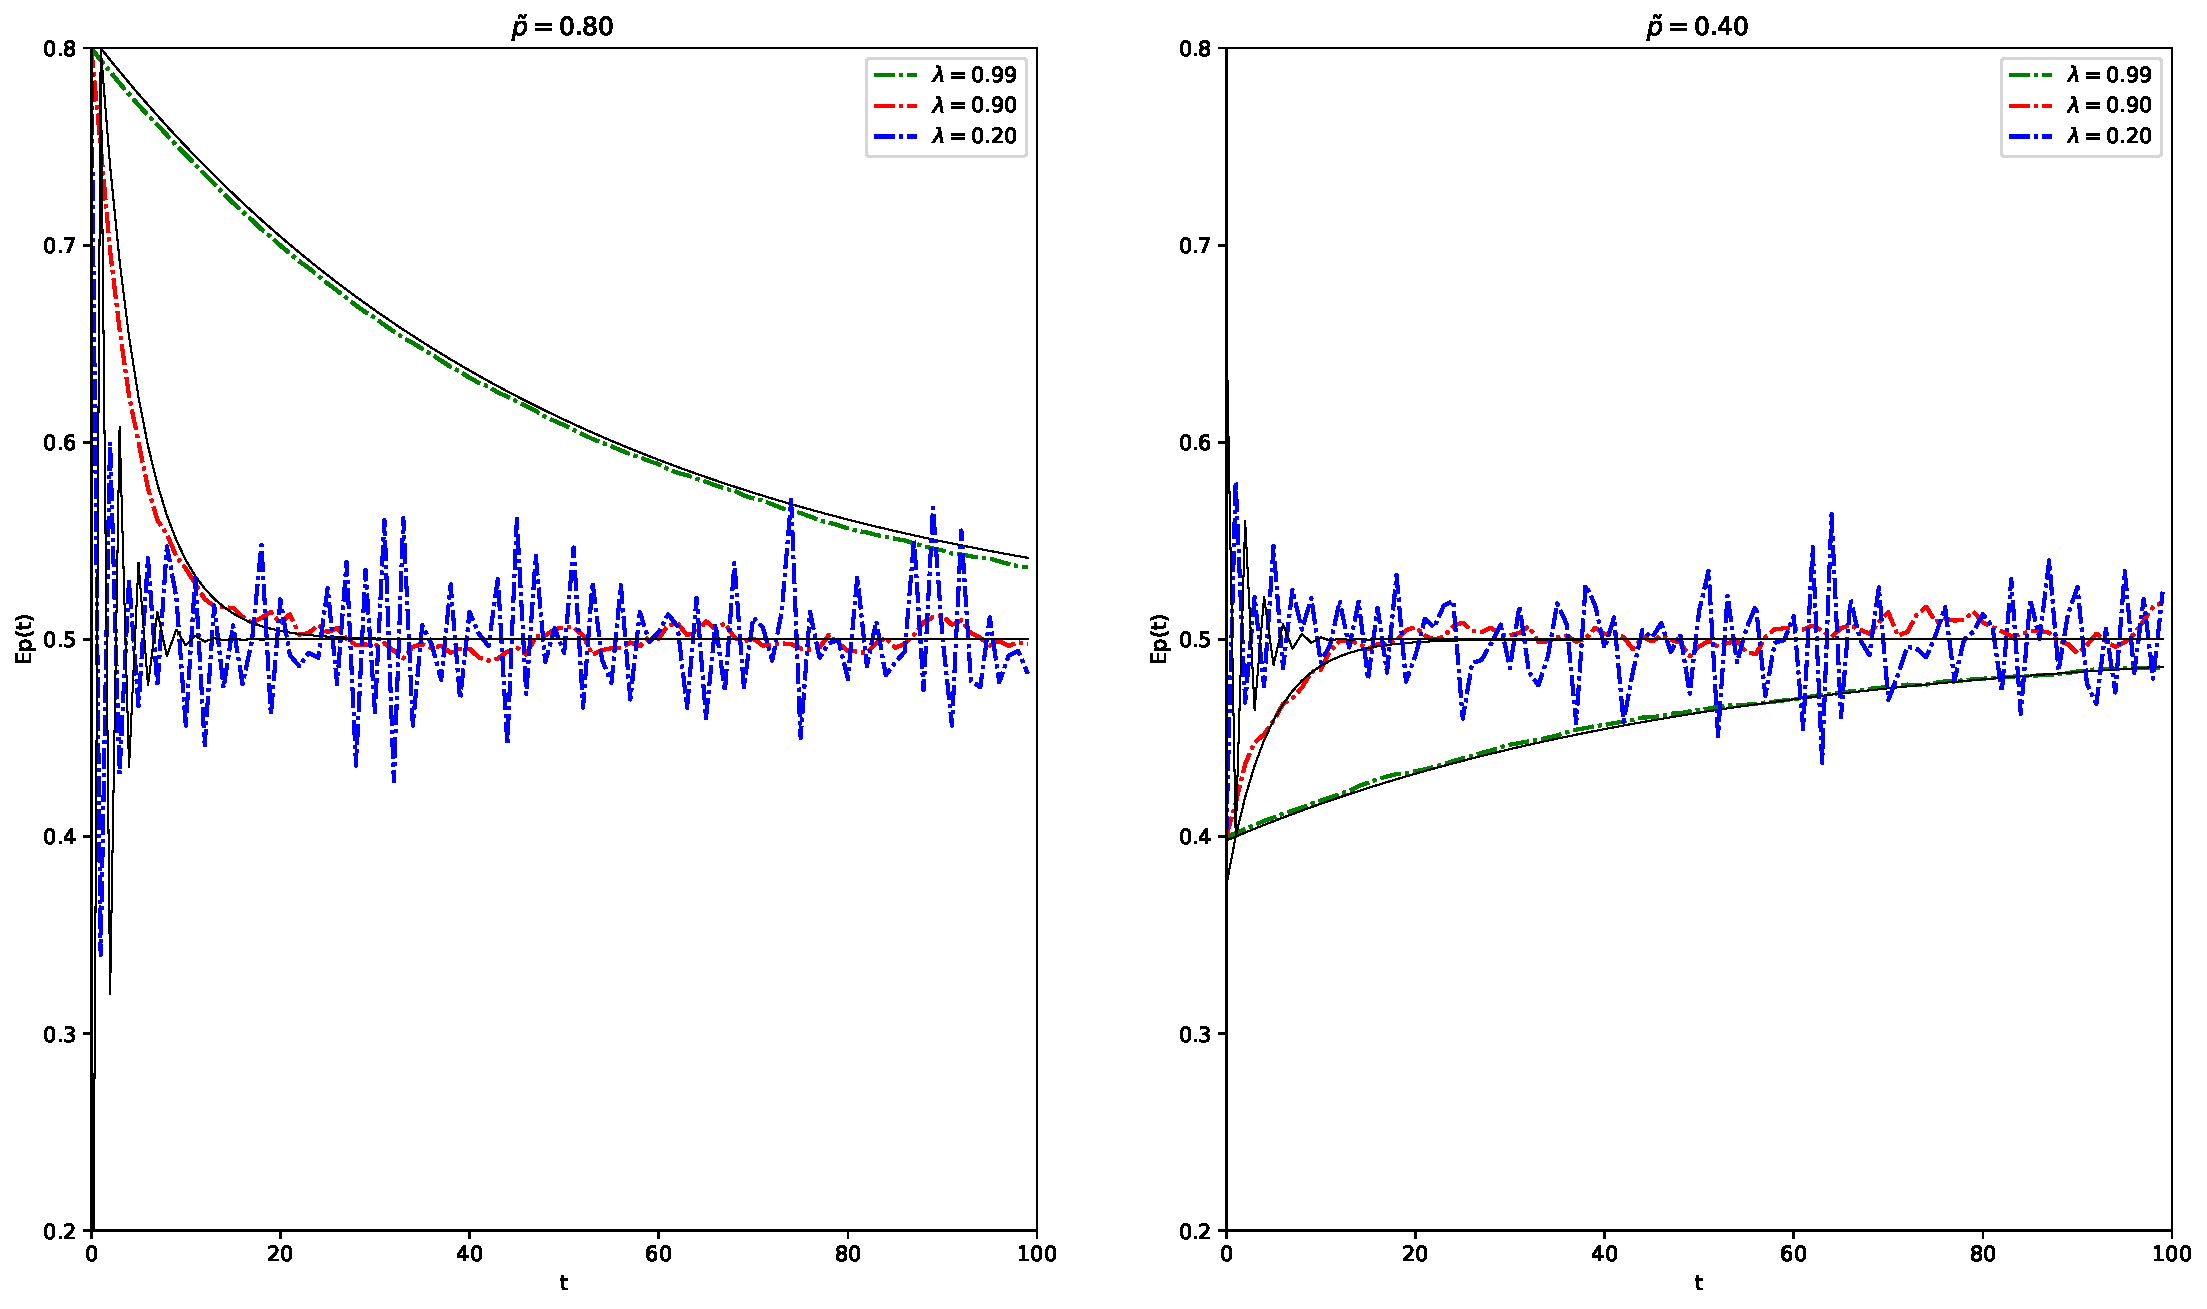
\includegraphics[width=1\textwidth]{Ept}
\end{frame}
%
\begin{frame}{Example - Transition probability variance}

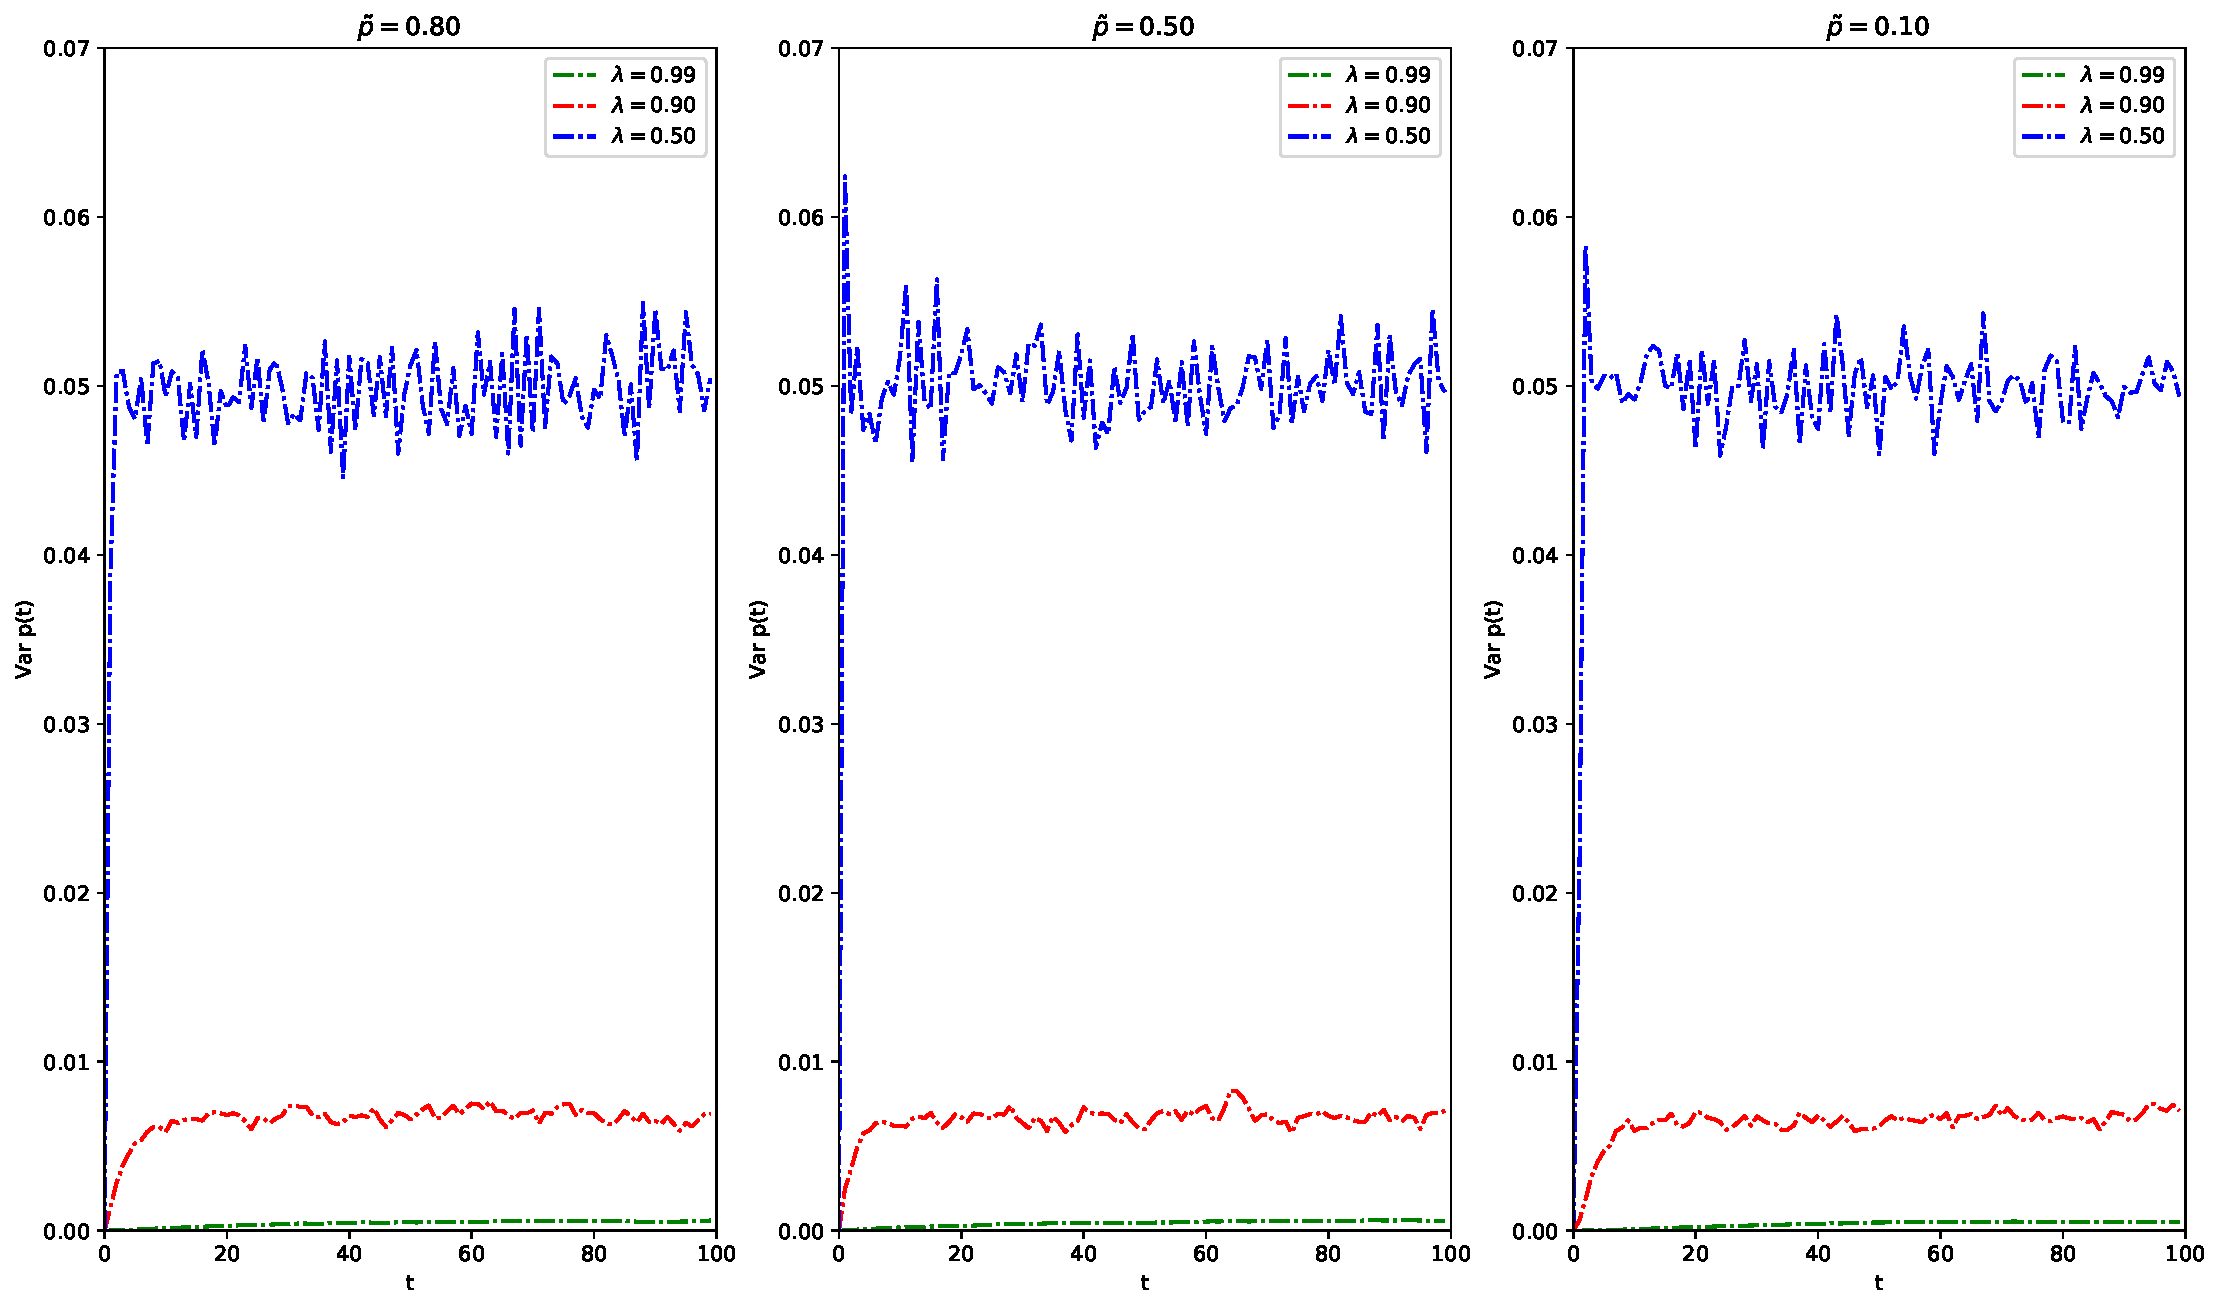
\includegraphics[width=1\textwidth]{Varpt}
\end{frame}
%
\begin{frame}{Example - Expected position of the walker}

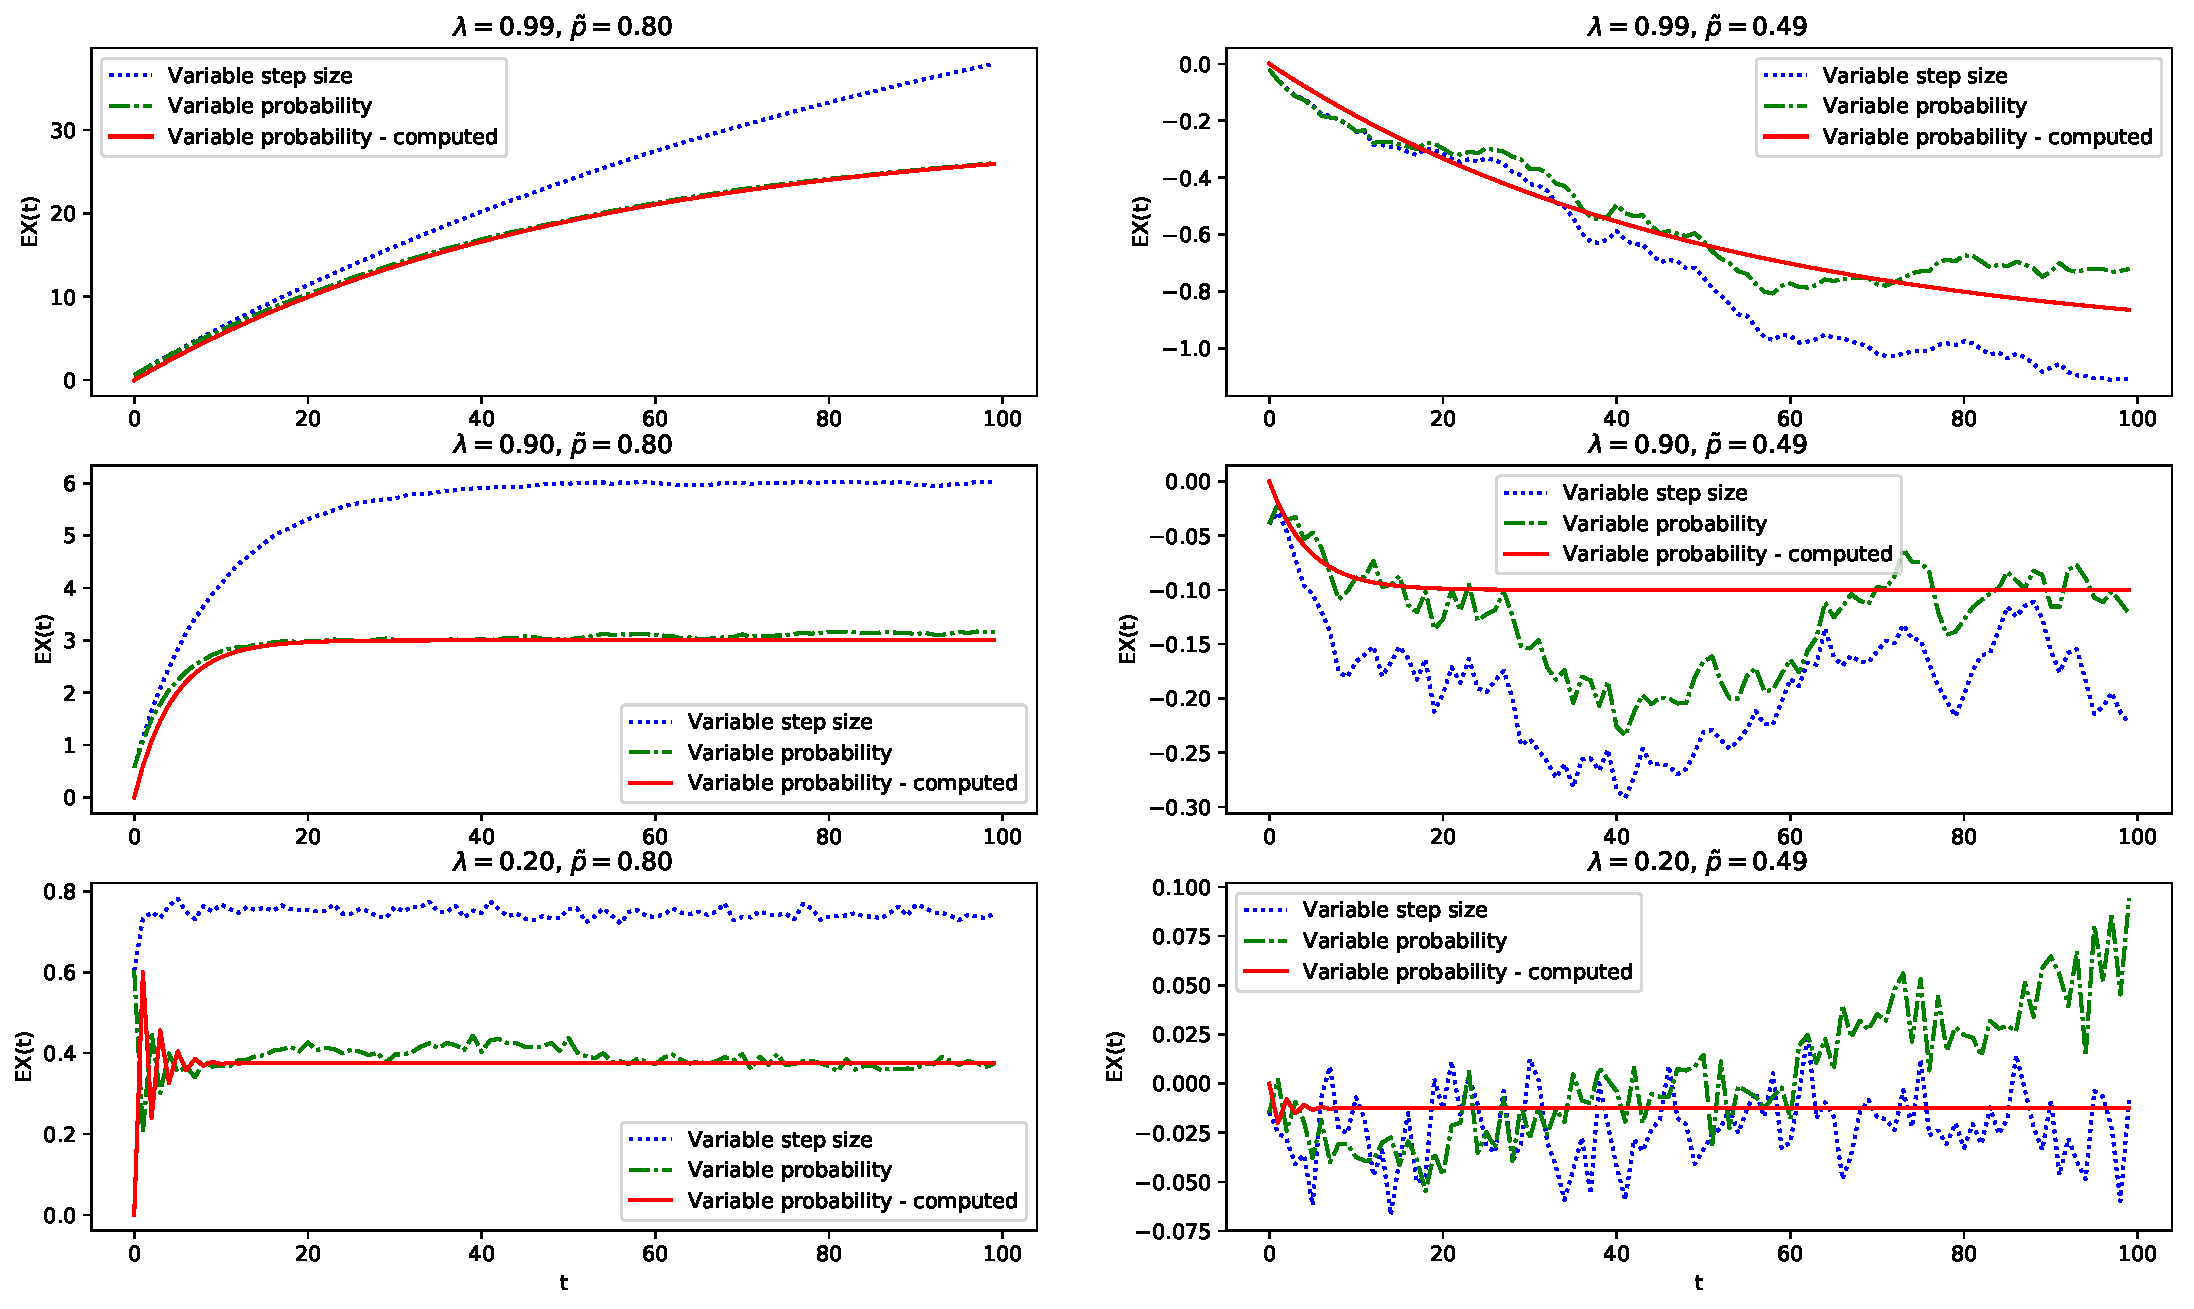
\includegraphics[width=1\textwidth]{EXt}
\end{frame}
%
\begin{frame}{Example - Walker's position variance}

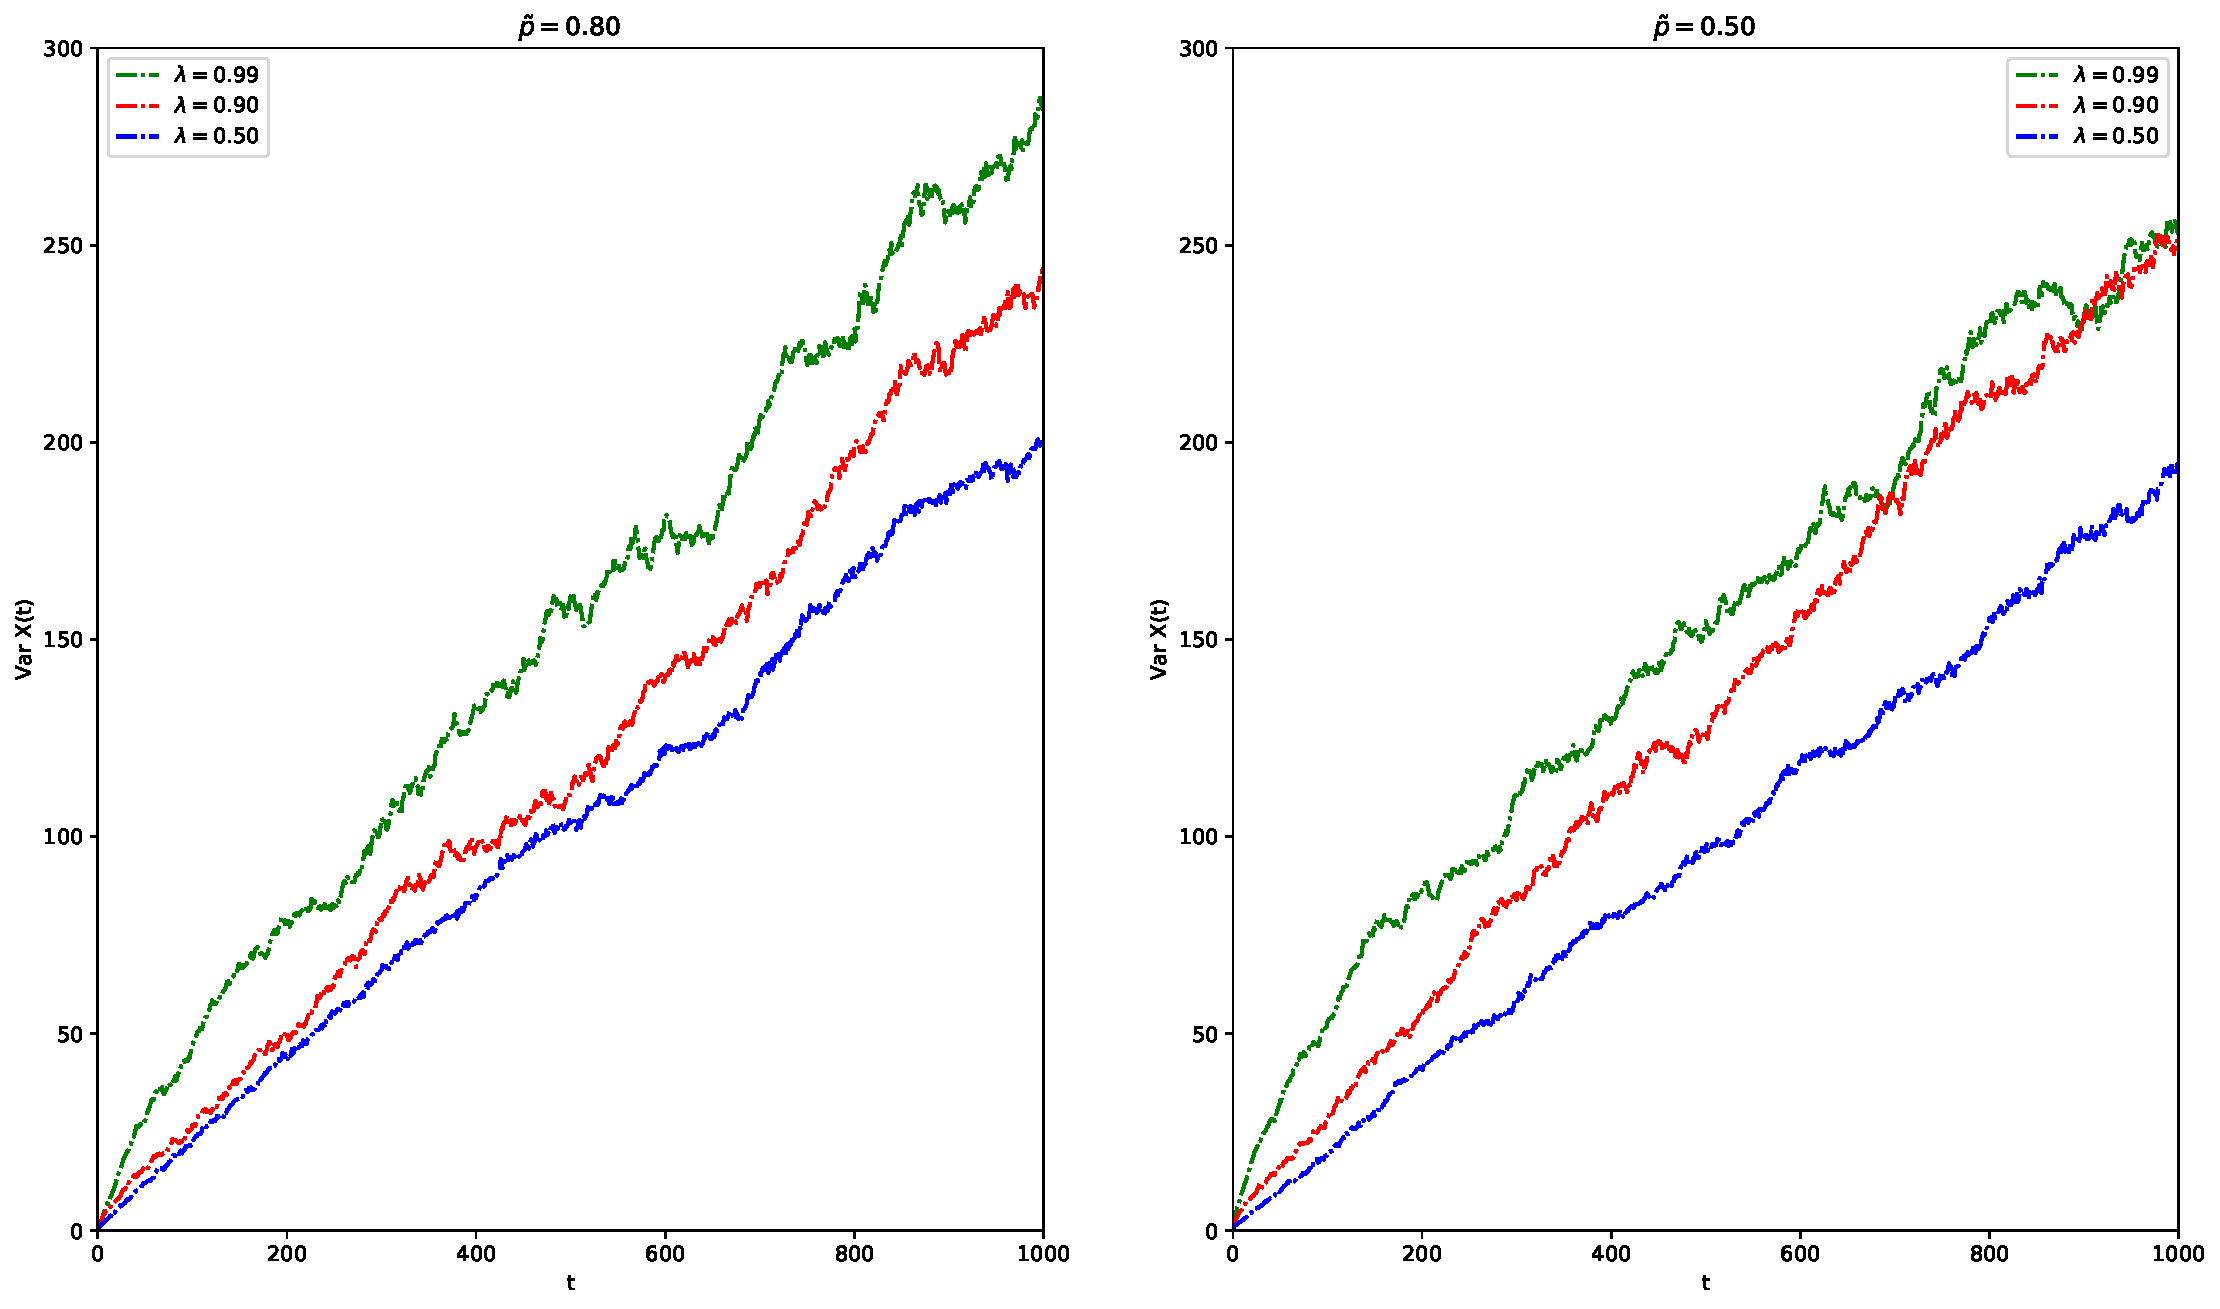
\includegraphics[width=1\textwidth]{VarXt}
\end{frame}
%
\begin{frame}{Alternative definitions}

\begin{itemize}
\item Formulas to obtain next transition probability $P_{i}$:
\begin{itemize}
\item<2-> $\frac{1}{2}[(1+X_{i})\lambda P_{i-1}+(1-X_{i})(1-\lambda(1-P_{i-1}))]$
\begin{itemize}
\item<3-> Success punished\medskip{}
\end{itemize}
\item<4-> $\frac{1}{2}[(1-X_{i})\lambda P_{i-1}+(1+X_{i})(1-\lambda(1-P_{i-1}))]$
\begin{itemize}
\item<5-> Success rewarded\medskip{}
\end{itemize}
\item<6-> $\frac{1}{2}[(1+X_{i})\lambda_{0}P_{i-1}+(1-X_{i})(1-\lambda_{1}(1-P_{i-1}))]$
\begin{itemize}
\item<6-> Success punished with multiple $\lambda$\medskip{}
\end{itemize}
\item<7-> $\frac{1}{2}[(1-X_{i})\lambda_{0}P_{i-1}+(1+X_{i})(1-\lambda_{1}(1-P_{i-1}))]$
\begin{itemize}
\item<7-> Success rewarded with multiple $\lambda$
\end{itemize}
\end{itemize}
\end{itemize}

\end{frame}
%
\begin{frame}{Data generation}
\begin{itemize}
\item Using Python \& Numpy package
\item Different parameters:
\begin{itemize}
\item $\lambda\in\{0.5,\,0.8,\,0.9,\,0.99\}$\medskip{}
\item $\bar{\lambda}=\{[0.5,\,0.8],\,[0.5,\,0.99],\,[0.99,\,0.9]\}$\medskip{}
\item $p_{0}=\{0.5,\,0.8,\,0.9,\,0.99\}$\medskip{}
\item $n=\{5,\,10,\,50,\,100\}$\medskip{}
\item $100$ walks for each combination
\end{itemize}
\end{itemize}
\end{frame}
%
\begin{frame}{Fitting parameters on generated data}

\begin{itemize}
\item Find $\overrightarrow{\lambda}$ with known $p_{0}$, model type
\item Find $p_{0}$ with known $\overrightarrow{\lambda}$, model type
\item Find $p_{0},\,\overrightarrow{\lambda}$ with known model type
\item Find model type without any prior knowledge
\end{itemize}
\end{frame}
%
\begin{frame}{Parameter fitting evaluation}

\begin{tabular}{|c|c|c|c|c|}
\hline 
 & SP - 1$\lambda$ & SR - 1$\lambda$ & SP - 2$\lambda$ & SR - 2$\lambda$\tabularnewline
\hline 
\hline 
Find $\overrightarrow{\lambda}$ & 96.9 \% & 34.4 \% & 80.2 \% & 77.1 \%\tabularnewline
\hline 
Find $p_{o}$ & 92.2 \% & 82.8 \% & 89.6 \% & 93.8 \%\tabularnewline
\hline 
Find $\overrightarrow{\lambda},\,p_{0}$ & 91.4 \% & 84.4 \% & 83.3 \% & 79.9 \%\tabularnewline
\hline 
Find model type & 1.6 \% & 1.6 \% & 87.5 \% & 89.6 \%\tabularnewline
\hline 
\end{tabular}
\end{frame}
%
\begin{frame}{Parameter fitting evaluation}

\begin{tabular}{|c|c|c|c|c|}
\hline 
 & SP - 1$\lambda$ & SR - 1$\lambda$ & SP - 2$\lambda$ & SR - 2$\lambda$\tabularnewline
\hline 
\hline 
Find $\overrightarrow{\lambda}$ & 96.9 \% & 34.4 \% & 80.2 \% & 77.1 \%\tabularnewline
\hline 
Find $p_{o}$ & 92.2 \% & 82.8 \% & 89.6 \% & 93.8 \%\tabularnewline
\hline 
Find $\overrightarrow{\lambda},\,p_{0}$ & 91.4 \% & 84.4 \% & 83.3 \% & 79.9 \%\tabularnewline
\hline 
Find model type & 93.8 \% & 87.5 \% & 89.6 \% & 89.6 \%\tabularnewline
\hline 
\end{tabular}
\end{frame}
%
\begin{frame}{Real life applications}

\begin{itemize}
\item Random processes with memory and one or just few dominant events
\begin{itemize}
\item Reliability analysis, medical data analysis, criminal recidivism
\item<2-> Sport modelling
\begin{itemize}
\item<3-> Tennis with model ``Success rewarded''
\item<3-> Applied for live betting on US Open against Tipsport bookmaker
\item<4-> Source code and paper available at https://github.com/tomaskourim/mathsport2019
\end{itemize}
\end{itemize}
\end{itemize}
\end{frame}
%
\begin{frame}{Summary}
\begin{itemize}
\item New models of Random walk described
\item Properties derived
\item Strenght of the models shown using simulated data
\item Possible real life applications shown
\item Source code and paper available at https://github.com/tomaskourim/amistat2019
\end{itemize}
\end{frame}
%
\begin{frame}{Next steps}
\begin{itemize}
\item More detailed model description
\begin{itemize}
\item Asymptotic behavior
\item Multidimensional models
\end{itemize}
\item<2-> Model improvement
\begin{itemize}
\item<2-> Other versions of random walk with memory
\item<2-> Combination with other approaches
\end{itemize}
\item<3-> Application in other domains
\end{itemize}
\end{frame}
%

\begin{frame}[plain] 
\begin{quote}%{} 
\begin{center} 
\huge{Thank you.} 
\end{center}
\vspace{10mm} 
\begin{center} 
\large{tom@skourim.com} 
\end{center}
\end{quote}%{} 
\end{frame}
\end{document}
